\chapter{Mobility, Resistivity, and the Hall Effect}
\label{ch:mobility-resistivity-hall}

The preceding chapters derived mobility from momentum relaxation and effective
mass.  A semiconductor measurement does not determine either quantity alone.
It measures the combined response of band structure, lattice scattering,
ionized impurities, and carrier populations.  This chapter completes the
low-field drift treatment of Sze and Lee, Chapter~2, by connecting mobility to
resistivity and Hall data \cite[Chap.~2]{szeLee2012}.

\section{Notation and units}

\begin{center}
\small
\begin{tabularx}{\textwidth}{@{}lX@{}}
\toprule
Symbol & Meaning and SI unit unless stated otherwise \\
\midrule
$q$ & Positive elementary-charge magnitude, measured in coulombs. \\
$\bm E$ & Electric field, measured in volts per meter. \\
$\bm B$ and $B_z$ & Magnetic flux density and its $z$ component, measured in teslas. \\
$n,p$ & Electron and hole number densities, measured in inverse cubic meters. \\
$m_n^*,m^*$ & Electron or generic conductivity effective mass, measured in kilograms. \\
$\tau_n,\tau,\tau_r$ & Electron, total, or mechanism-specific momentum-relaxation time, measured in seconds; $r$ labels a scattering mechanism. \\
$\bm v_{n,\mathrm d},v_{\mathrm{th}},\ell$ & Electron drift velocity and thermal speed in meters per second, and mean free path in meters. \\
$\mu,\mu_n,\mu_p,\mu_{\mathrm L},\mu_{\mathrm I},\mu_r$ & Total, electron, hole, lattice-limited, impurity-limited, or mechanism-specific mobility, measured in square meters per volt-second. \\
$T,\kb$ & Absolute temperature in kelvin and Boltzmann constant in joules per kelvin. \\
$N_{\mathrm I}$ & Total ionized-impurity density, measured in inverse cubic meters. \\
$\bm J,J_x,I_x$ & Current density in amperes per square meter, its $x$ component, and total $x$-directed current in amperes. \\
$\sigma,\rho$ & Conductivity in siemens per meter and resistivity in ohm-meters. \\
$t,R_{\square}$ & Sample thickness in meters and sheet resistance in ohms per square. \\
$E_y,V_H,R_H$ & Hall field in volts per meter, Hall voltage in volts, and Hall coefficient in cubic meters per coulomb. \\
$\mu_H$ & Hall mobility, measured in square meters per volt-second. \\
\bottomrule
\end{tabularx}
\end{center}

\section{Scattering-limited mobility}

For an isotropic parabolic band, the low-field drift velocity and mobility are
\begin{equation}
  \bm v_{n,\mathrm d}=-\mu_n\bm E,
  \qquad
  \mu_n=\frac{q\tau_n}{m_n^*},
  \label{eq:measured-electron-mobility}
\end{equation}
with the analogous positive drift relation for holes.  The thermal speed and
mean free path provide separate microscopic scales,
\begin{equation}
  v_{\mathrm{th}}=\sqrt{\frac{3\kb T}{m^*}},
  \qquad
  \ell=v_{\mathrm{th}}\tau.
  \label{eq:transport-thermal-speed-path}
\end{equation}
Thermal motion is much faster than the low-field drift motion.  Mobility
measures the small field-induced displacement of an otherwise randomized
velocity distribution.

Lattice vibrations and ionized impurities produce distinct temperature trends.
A reduced nondegenerate model gives
\begin{equation}
  \mu_{\mathrm L}\propto T^{-3/2},
  \qquad
  \mu_{\mathrm I}\propto \frac{T^{3/2}}{N_{\mathrm I}}.
  \label{eq:transport-mobility-power-laws}
\end{equation}
Independent momentum-relaxation rates add.  Therefore
\begin{equation}
  \frac1\tau=\sum_r\frac1{\tau_r},
  \qquad
  \boxed{\frac1\mu=\sum_r\frac1{\mu_r}.}
  \label{eq:transport-matthiessen}
\end{equation}
This Matthiessen construction explains why lightly doped material is
lattice-limited at high temperature and heavily doped material is
impurity-limited at low temperature.  The power laws are asymptotic teaching
models rather than universal mobility formulas.

\section{Conductivity and resistivity}

Electron and hole drift currents add as conventional current:
\begin{equation}
  \bm J_{\mathrm{drift}}
  =q(n\mu_n+p\mu_p)\bm E.
  \label{eq:transport-total-drift-current}
\end{equation}
The conductivity and resistivity are
\begin{equation}
  \boxed{\sigma=q(n\mu_n+p\mu_p),}
  \qquad
  \boxed{\rho=\frac1\sigma.}
  \label{eq:transport-conductivity-resistivity}
\end{equation}
In a majority-electron sample, $\rho\simeq(qn\mu_n)^{-1}$.  Increasing donor
density raises $n$ but also strengthens ionized-impurity scattering and lowers
$\mu_n$.  Resistivity therefore cannot be converted into dopant density without
a mobility model and an ionization model.

A four-point probe separates current injection from voltage measurement.  For
a thin sheet with thickness $t$, the sheet resistance is $R_{\square}=\rho/t$.
Geometric correction factors convert the measured voltage-to-current ratio
into $R_{\square}$.  The measurement determines resistivity; carrier type and
carrier density require Hall information.

\section{Hall response}

Let current flow along $x$ and apply $\bm B=B_z\hat{\bm z}$.  Transverse charge
accumulation creates a Hall field until the transverse Lorentz force vanishes.
For one dominant carrier type,
\begin{equation}
  E_y=R_HJ_xB_z,
  \label{eq:transport-hall-field}
\end{equation}
where
\begin{equation}
  \boxed{
  R_H=-\frac1{qn}\quad\text{for electrons},
  \qquad
  R_H=+\frac1{qp}\quad\text{for holes}.
  }
  \label{eq:transport-hall-coefficients}
\end{equation}
For a rectangular sample of thickness $t$ carrying total current $I_x$,
\begin{equation}
  V_H=\frac{R_H I_xB_z}{t}.
  \label{eq:transport-hall-voltage}
\end{equation}
The sign identifies the dominant mobile charge.  The magnitude gives the
one-carrier density, and the combination of Hall density and conductivity gives
the Hall mobility,
\begin{equation}
  \mu_H=|R_H|\sigma.
  \label{eq:transport-hall-mobility}
\end{equation}
A Hall scattering factor relates $\mu_H$ to the drift mobility when the
relaxation time depends on carrier energy.  Multicarrier conduction replaces
\cref{eq:transport-hall-coefficients} by a mobility-weighted expression, so a
single inverse Hall coefficient no longer equals the total carrier density.

\begin{figure}[htbp]
  \centering
  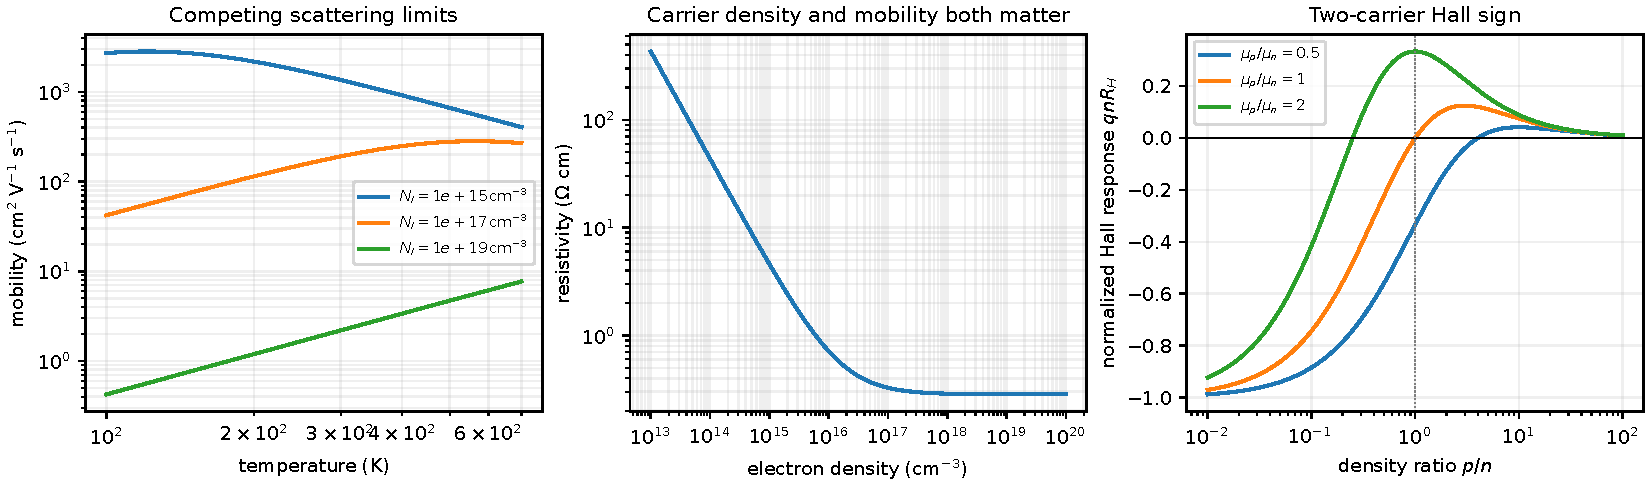
\includegraphics[width=\textwidth]{figures/transport-mobility-hall.pdf}
  \caption{Competing lattice and impurity mobility limits, the resulting
  resistivity trend, and the opposite Hall signs of electron and hole
  conduction.\figurenotebookmark}
  \label{fig:transport-mobility-hall}
\end{figure}
\figurenotebooktext{figures/12_mobility-resistivity-hall/fig_12_01.ipynb}

\section{Range of validity}

The scalar formulas assume one isotropic band, low electric field, and a single
dominant carrier type.  Tensor bands require tensor conductivity and Hall
response.  Degenerate statistics require Fermi-window averages of the
energy-dependent scattering time.  Strong magnetic fields require the full
magnetoconductivity tensor.  The empirical power laws in
\cref{eq:transport-mobility-power-laws} identify trends but do not replace
measured or microscopic scattering models.

\section{Chapter summary}

Effective mass converts momentum relaxation into mobility.  Lattice and
ionized-impurity scattering contribute additive inverse mobilities.
Conductivity combines carrier density and mobility, whereas Hall data separate
carrier sign and an effective one-carrier density.  These measurements provide
the transport parameters needed by the drift--diffusion equations.
